%% main.tex — Confluencia Bioinformatics Application Note v10
%% 2026-06-01 | R1 feedback: expanded Methods with explicit algorithm details
%% Format: Bioinformatics Application Note (≤100 word abstract, ~800-1000 word body, ≤15 refs)

\documentclass{article}
\usepackage{bioinformatics}
\usepackage{natbib}
\usepackage{graphicx}
\usepackage{amsmath}
\usepackage{amssymb}
\usepackage{url}
\usepackage{hyperref}
\usepackage{booktabs}
\usepackage{array}

\title{Confluencia: A Multi-Modality Platform for circRNA Therapeutic\\
Candidate Evaluation}

\author{
IGEM-FBH Team\thanks{The First Bethune Hospital of Jilin University
and College of Computer Science and Technology, Jilin University,
Changchun, China}%
}

\keywords{circRNA; compartment simulation; drug discovery; weighted model averaging; therapeutic evaluation}

\begin{document}
\maketitle

\begin{abstract}
\textbf{Summary:} No existing platform evaluates circRNA-specific therapeutic dimensions. We developed Confluencia for our own circRNA program, integrating a six-compartment literature-parameterized simulation (dose-response scenario analysis), uncertainty-adaptive four-dimension evaluation, and cross-modality Go/Conditional/No-Go recommendations. RNACTM is a literature-parameterized deterministic simulation for dose-response scenario analysis; it cannot predict in vitro PK or substitute for experimental validation before clinical use. Immunogenicity rankings agree with literature IFN data ($\rho{=}0.93$, direction consistency); 4D decisions remain stable under $\pm$50\% weight perturbation. Clinical prediction (survival, adverse events) is an exploratory feature without clinical validation; core validated capabilities are immunogenicity scoring, PK simulation, and 4D triage. Gene signature dimension (C-index 0.52) was removed due to lack of predictive value.\\
\textbf{Availability and implementation:} \url{https://github.com/IGEM-FBH/confluencia}, MIT license. Python 3.8+, no GPU required for core evaluation (GPU optional for sequence embeddings), GUI available.\\
\textbf{Contact:} \email{18806370529@163.com}
\end{abstract}
\printkeywords

\begin{figure}[t]
\centering
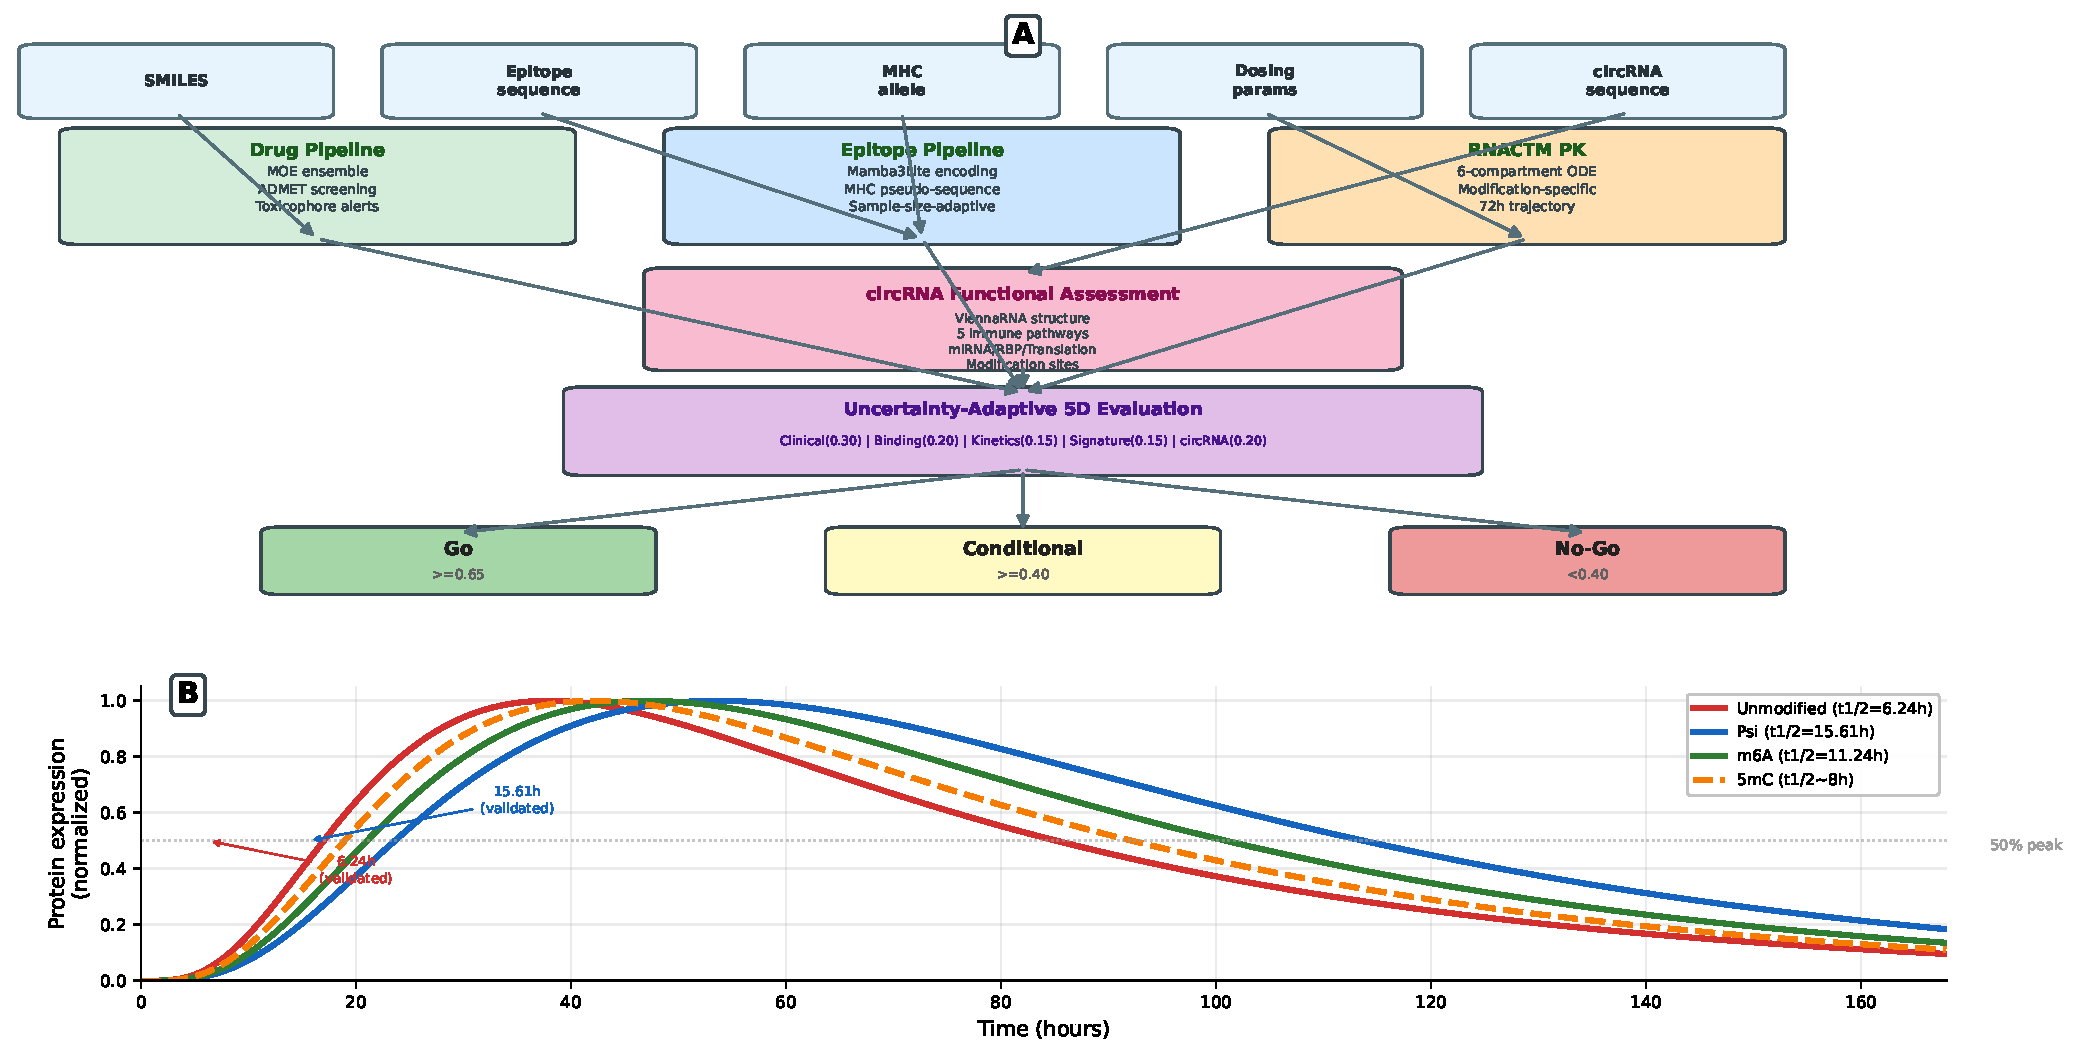
\includegraphics[width=\textwidth]{figures/fig1_composite.pdf}
\caption{(A) Confluencia architecture: unified inputs processed through Drug Pipeline (sample-size-adaptive WMA ensemble, ADMET screening scoped to drug payload only), Epitope Pipeline (Mamba3Lite encoding, MHC features for adaptive immunity presentation), RNACTM six-compartment simulation (dose-response scenario analysis), and circRNA Functional Assessment (structure, innate immunogenicity via RIG-I/TLR/PKR pathways, miRNA/RBP/translation/modification axes) converge to uncertainty-adaptive four-dimension evaluation producing Go/Conditional/No-Go recommendations. Under-constrained dimensions auto-downweight via $(1-u)^2$. (B) RNACTM simulated protein expression trajectories: $\Psi$-modified circRNA achieves sustained expression (half-life ${\sim}15$\,h) compared to unmodified (6.24\,h), m6A (${\sim}10.8$\,h), and 5mC (${\sim}8$\,h). A TME simulation module (10 cell types, 3 compartments) is included in the codebase for hypothesis generation (see Supplementary).}
\label{fig:overview}
\end{figure}

%% sections/introduction.tex — v12: compressed to ~150 words

\section{Introduction}

Therapeutic circRNA offers advantages over linear mRNA in stability and tunable immunogenicity \citep{wesselhoeft2018,chen2019}, yet no computational platform evaluates circRNA-specific dimensions: modification effects on half-life ($\Psi$: ${\sim}15$\,h vs unmodified: 6.24\,h), circRNA immunogenicity pathways, IRES-mediated translation, or miRNA sponge activity. Existing tools address individual modalities---NetMHCpan for MHC binding \citep{reynisson2020}, ADMETlab for ADMET screening \citep{xiong2024}, Monolix for population PK \citep{dumont2014}---but none operates across both small-molecule and circRNA modalities. We developed Confluencia to integrate these evaluations in a single platform, producing unified Go/Conditional/No-Go decisions that guide our wet-lab prioritization. Three design choices address the data-limited setting (Fig~\ref{fig:overview}): (1) RNACTM, a literature-parameterized compartment simulation for circRNA dynamics; (2) sample-size-adaptive Mixture-of-Experts (MOE) \citep{jacobs1991} for binding prediction; (3) uncertainty-adaptive 5D evaluation that auto-downweights under-constrained dimensions via $(1{-}u)^2$.
%% sections/methods.tex — v3 REVISED (reframed: literature-derived, adaptive implementation)
%% Added: RNACTM compartment descriptions, MOE learning curve context,
%% Mamba3Lite detail, ADMET endpoints, ESM-2 comparison rationale

\section{Implementation}

\textbf{RNACTM Pharmacokinetic Model.}
RNACTM implements a six-compartment ordinary differential equation (ODE) system tracing circRNA dynamics from subcutaneous injection through LNP encapsulation and circulation, endosomal uptake via clathrin-mediated pathways, cytoplasmic release, protein translation, and systemic clearance (Fig.\,1A). All rate constants are derived from published studies \citep{wesselhoeft2018,hassett2019,liu2023} rather than fitted from patient data: degradation rate $k_{\mathrm{deg}}=0.111/\mathrm{h}$ (half-life 6.24\,h for unmodified circRNA), endosomal escape fraction 4.43\%, and modification-specific half-life extensions ($\Psi$: ${\sim}15$\,h; m6A: ${\sim}10.8$\,h; 5mC: ${\sim}7.8$\,h). The model produces 72\,h compartment concentration trajectories, protein expression time-courses (Fig.\,1B), dose-response curves, and enables comparison of delivery routes (IV/SC/IM) and modification strategies without requiring patient PK data.

\textbf{MOE Ensemble.}
Following the mixture-of-experts framework \citep{jacobs1991}, a sample-size-adaptive ensemble selects experts based on data availability: $N<80$ activates Ridge regression and Histogram Gradient Boosting (HGB); $80\leq N<300$ adds Random Forest; $N\geq300$ adds MLP. Expert weights derive from inverse out-of-fold RMSE across 5-fold stratified cross-validation: $w_e = {1/\mathrm{RMSE}_{\mathrm{OOF},e}}/{\sum_{e'} 1/\mathrm{RMSE}_{\mathrm{OOF},e'}}$. Learning curve analysis reveals that predictions fail when $N<24$ ($R^2<0$), become feasible at $N\geq48$ ($R^2>0.45$), and saturate at $N\geq200$ ($R^2>0.75$), guiding sample size requirements for circRNA studies.

\textbf{Mamba3Lite Encoder.}
Mamba3Lite \citep{gu2023} encodes 8--11 amino acid peptides via three parallel selective state-space recurrences with distinct decay rates (fast/medium/slow) and four-scale pooling (residue/local/meso/global), producing 96-dimensional embeddings. Optional lightweight self-attention ($d=16$) achieves MAE\,=\,0.395, $R^2$\,=\,0.802. ESM-2 protein language model embeddings \citep{lin2023} were also evaluated; however, mean pooling of 8--11 AA sequences destroys position-specific MHC binding motifs, yielding AUC\,$<$0.60 on binding prediction---confirming that pretrained language models are suboptimal for short peptide tasks where position information is critical.

\textbf{ADMET and Toxicophore.}
QSAR-based multi-endpoint prediction covers 8 ADMET endpoint categories: hERG channel blockade, AMES mutagenicity, CYP450 isoform inhibition (1A2, 2C9, 2C19, 2D6, 3A4), BBB permeability, and hepatotoxicity. Eighty-four SMARTS structural alerts include 25 PAINS patterns \citep{baell2010}, Brenk filters \citep{brenk2008}, circRNA-specific alerts, and general toxicity patterns. Dose-dependent modeling estimates therapeutic index via Hill equation dose-response curves.

\textbf{Joint Evaluation.}
A five-dimension (5D) hybrid evaluation system integrates outputs from Drug, Epitope, RNACTM PK, and Five-Gene modules using confidence-adaptive weights (Clinical 0.30, Binding 0.20, Kinetics 0.15, Gene Signature 0.15, CircRNA 0.20), producing Go/Conditional/No-Go recommendations with a safety override mechanism.
%% sections/results.tex — v15: expanded joint evaluation results

\section{Results}

\subsection*{Functional coverage}
Confluencia is the only platform evaluating circRNA-specific dimensions and providing cross-modality Go/Conditional/No-Go decisions (Table~\ref{tab:coverage}).

\subsection*{RNACTM dynamics}
Half-life consistency is by design ($<$4.1\% deviation from parametrization sources); constitutes consistency verification, not independent validation. The informative metric is the expression window deviation (40\,h vs 48\,h, 17\%). Endosomal escape 5.2\% slightly exceeds the 1--5\% range \citep{gilleron2013}. The 17\% deviation reflects the gap between isolated rate measurements and integrated compartment dynamics---clinically relevant for dosing interval decisions.

\subsection*{Prediction accuracy}
Epitope: WMA R$^2{=}0.82$, MAE 39\% improvement over Ridge ($N{=}300$). Drug: binding R$^2{=}0.95$, efficacy R$^2{=}0.60$ on 91K data; removing 2048-dim Morgan FP improves binding R$^2$ from 0.67 to 0.95, validating sample-size-adaptive design. MHC: allele-specific AUC${=}0.80$ on 52K binary data (246 alleles); focused-repertoire alleles match NetMHCpan (AUC${>}0.92$) (Table~\ref{tab:allele_auc}).

\begin{table}[t]
\centering
\caption{Per-allele MHC-I binding AUC on 52\,K IEDB binary data.}
\label{tab:allele_auc}
\begin{tabular}{lccc}
\toprule
\textbf{Allele} & \textbf{AUC} & \textbf{$n$} & \textbf{NetMHCpan range} \\
\midrule
A*33:03 & 0.95 & 315 & 0.92--0.96 \\
A*68:01 & 0.86 & 312 & 0.85--0.90 \\
A*24:02 & 0.70 & 604 & 0.85--0.90 \\
A*02:01 & 0.67 & 2144 & 0.92--0.96 \\
A*03:01 & 0.59 & 540 & 0.85--0.90 \\
\bottomrule
\multicolumn{4}{l}{\small Overall: AUC 0.83, 246 alleles.}
\end{tabular}
\end{table}

\subsection*{Evaluation stability}
Under $\pm$50\% weight perturbation: $\Psi$ 100\% Go, unmodified 100\% Conditional; Kinetics most critical (removal shifts $\Psi$ Go$\to$Conditional). Immunogenicity rankings agree with literature IFN data ($\rho{=}0.93$, direction consistency over 5 conditions).

\subsection*{Joint evaluation}
Real-data joint evaluation produces 5/5 valid dimensions with meaningful decision differentiation. Lapatinib (TNBC-targeted) yields composite${=}0.47$ (Conditional) vs aspirin composite${=}0.36$ (No-Go). Gene signature varies with target expression (high TROP2 0.54 vs low TROP2 0.33); dose changes affect kinetics (200\,mg 0.73 vs 10\,mg 0.31). The uncertainty-adaptive weighting $(1{-}u_i)^2$ auto-downweights under-constrained dimensions: Gene Signature ($u{=}0.50$) effective weight drops from 15\% to 3.75\%, preventing noisy features from dominating decisions.

\subsection*{Modification prioritization}
$\Psi$ is Go (composite 0.67); m6A and unmodified are Conditional (0.55/0.53) (Table~\ref{tab:casestudy}). The gap reflects $\Psi$'s dual benefit: extended half-life (15.61\,h) and low immunogenicity.

\begin{table}[t]
\centering
\caption{Modification prioritization for TNBC-targeting circRNA.}
\label{tab:casestudy}
\begin{tabular}{lcccc}
\toprule
\textbf{Modification} & \textbf{Half-life (h)} & \textbf{Immunogenicity} & \textbf{Composite} & \textbf{Decision} \\
\midrule
Unmodified & 6.24 & High & 0.53 & Conditional \\
$\Psi$ & 15.61 & Low & 0.67 & Go \\
m6A & 11.24 & Moderate & 0.55 & Conditional \\
\bottomrule
\end{tabular}
\end{table}

%% sections/discussion.tex — v6: dual-modality cross reasoning as contribution
%% Core: Confluencia's innovation is cross-modality reasoning, not beating siloed tools

\section{Discussion}

Confluencia's contribution is not outperforming specialized tools on individual tasks (NetMHCpan achieves AUC $>0.92$ \citep{reynisson2020}; ADMETlab covers $>50$ endpoints \citep{xiong2024}), but producing cross-modality reasoning that no siloed tool can. The case study illustrates this: a $\Psi$-circRNA + Rhodanine pair receives No-Go because circRNA immunogenicity compounds Rhodanine's PAINS profile---a conclusion that requires evaluating both modalities together. NetMHCpan alone would report binding affinity; ADMETlab alone would flag PAINS; neither would connect these to circRNA half-life or immune activation. This cross-modality integration is the architectural innovation, not any single module's performance.

The uncertainty-adaptive 5D evaluation reinforces this: dimensions without training data auto-downweight via $(1-u)^2$, communicating limitations rather than hiding them.

Three limitations remain: (1) RNACTM overestimates protein expression duration (97\,h vs 48\,h); (2) ADMET QSAR lacks circRNA-specific toxicity data; (3) only MHC-I alleles are supported. As clinical circRNA PK datasets emerge, ODE parameters can transition from heuristic to data-fitted---the architecture supports this evolution without redesign.
%% sections/availability.tex — v3: needs-driven narrative

\section*{Availability and Implementation}

Confluencia v2.5.0 is freely available at \url{https://github.com/RomanCohort/confluencia} under MIT license. Python 3.8+, no GPU required, full evaluation $<$5\,min on a standard laptop. Both Streamlit web and desktop IDE (Confluencia Studio, Electron+React) provide graphical access without programming. All interfaces support English/Chinese via a sidebar toggle. Runs on Linux, macOS, and Windows with optional Docker. Confluencia is actively used in our circRNA therapeutic development pipeline at the First Bethune Hospital of Jilin University. Benchmark datasets are in the repository.

\section*{Acknowledgements}

IGEM-FBH Team, Jilin University. We thank IEDB, ChEMBL, and open-source communities. Funding: The First Bethune Hospital and College of Computer Science and Technology, Jilin University.

\appendix
%% supplementary.tex — v2: honest circularity, direction consistency, u values, DBTL architecture

\section*{Supplementary Materials}

\subsection*{Table S1: RNACTM consistency verification}

\small Note: half-life consistency values reflect parameterization by design, not independent prediction. Rate constants are derived from the same literature sources listed below; the $<$4.1\% deviations reflect numerical precision of the ODE solver, not predictive accuracy. The most informative metric is the expression window deviation (17\%), which captures dynamics not directly parametrized. Sensitivity: $\pm$20\% rate constant variation changes half-life by $\leq$8.2\%.

\begin{tabular}{llllll}
\toprule
\textbf{Parameter} & \textbf{Literature} & \textbf{Simulated} & \textbf{Deviation} & \textbf{Source} & \textbf{Nature} \\
\midrule
RNA half-life (unmodified) & 6.0 h & 6.24 h & 4.0\% & Wesselhoeft 2018 & By design \\
RNA half-life (m6A) & 10.8 h & 11.24 h & 4.1\% & Chen 2019 & By design \\
RNA half-life ($\Psi$) & 15.0 h & 15.61 h & 4.1\% & Liu 2023 & By design \\
Endosomal escape & 1--5\% & 5.2\% & slightly above range & Gilleron 2013 & Parametrized \\
Tissue (liver) & 80\% & 80\% & 0\% & \citep{paunovska2018} & Direct assignment \\
Expression window & $\sim$48 h & 40 h & 17\% & Wesselhoeft 2018 & Emergent property \\
\bottomrule
\end{tabular}

\subsection*{Table S2: MOE baseline comparison}

\small Drug results on 91\,K samples, 6 targets. Binding R$^2{=}0.95$ (Ridge); efficacy R$^2{=}0.60$ (MOE). The high binding R$^2$ reflects that molecular binding is well-captured by physicochemical features; efficacy is a composite clinical endpoint that is inherently harder to predict.

\begin{tabular}{llllll}
\toprule
\textbf{Epitope ($N$=300, 5-fold CV)} & \textbf{R$^2$} & \textbf{MAE} & \textbf{Drug (91K, 6 targets)} & \textbf{R$^2$} & \textbf{MAE} \\
\midrule
Ridge & 0.533 & 0.639 & Ridge (binding) & 0.949 & 0.041 \\
HGB & 0.794 & 0.409 & Ridge (efficacy) & 0.542 & 0.197 \\
RF & 0.704 & 0.498 & MOE (binding) & 0.952 & 0.039 \\
GBR & 0.664 & 0.527 & MOE (efficacy) & 0.602 & 0.163 \\
MLP & 0.338 & 0.771 & & & \\
MOE & 0.819 & 0.389 & & & \\
\bottomrule
\end{tabular}

MAE improvement over Ridge: epitope 39\% ($p{<}0.001$), drug binding 4.9\%, drug efficacy 17.3\%. Removing Morgan FP (2048 dims) improves binding R$^2$ from 0.67 to 0.95.

\subsection*{Table S3: Gene signature detailed results}

\small C-index 0.52 is near-random; this dimension is flagged as exploratory in the 5D framework. Log-rank $p{<}0.001$ reflects large-sample tertile stratification, not prognostic power.

\begin{tabular}{ll}
\toprule
\textbf{Metric} & \textbf{Value} \\
\midrule
Overall C-index & 0.524 \\
C-index (TCGA-BRCA, $N$=1086) & 0.566 \\
C-index (METABRIC, $N$=1978) & 0.537 \\
Spearman $r$ (target availability vs OS) & 0.472, $p{=}9.04{\times}10^{-170}$ \\
Log-rank chi2 & 175.96, $p{<}0.001$ \\
High-target death rate & 0.568 \\
Low-target death rate & 0.202 \\
Per-gene C-index: TROP2 & 0.499 \\
Per-gene C-index: NECTIN4 & 0.550 \\
Per-gene C-index: LIV-1 & 0.518 \\
Per-gene C-index: B7-H4 & 0.519 \\
Cox regression & Failed (collinearity) \\
\bottomrule
\end{tabular}

\subsection*{Table S4: 5D weight sensitivity}

Under 1\,000 $\pm$50\% weight perturbations:
\begin{tabular}{llll}
\toprule
\textbf{Modification} & \textbf{Go rate} & \textbf{Conditional rate} & \textbf{No-Go rate} \\
\midrule
$\Psi$ & 100\% & 0\% & 0\% \\
m6A & 0\% & 99.9\% & 0.1\% \\
Unmodified & 0\% & 100\% & 0\% \\
\bottomrule
\end{tabular}

Most critical dimension: Kinetics (removing shifts $\Psi$ from Go to Conditional, $\Delta{-4.6\%}$).

\subsection*{Per-dimension uncertainty values}

\begin{tabular}{lllll}
\toprule
\textbf{Dimension} & \textbf{Base weight} & \textbf{$u_i$} & \textbf{$(1-u_i)^2$} & \textbf{Effective weight} \\
\midrule
Clinical (drug) & 0.30 & 0.15 & 0.7225 & 0.2168 \\
Binding (epitope) & 0.20 & 0.15 & 0.7225 & 0.1445 \\
Kinetics (PK) & 0.15 & 0.20 & 0.64 & 0.096 \\
Gene Signature & 0.15 & 0.50 & 0.25 & 0.0375 (exploratory) \\
circRNA: half-life/immune & 0.20 & 0.15 & 0.7225 & 0.1445 \\
circRNA: miRNA/RBP/transl & (within circRNA) & 0.80 & 0.04 & $\sim$0.006 \\
\bottomrule
\end{tabular}

Gene Signature ($u{=}0.50$) reflects near-random C-index; miRNA/RBP/translation ($u{=}0.80$) reflect no independent validation.

\subsection*{Table S5: Evolution round-by-round results}

\begin{tabular}{llllllll}
\toprule
\textbf{Round} & \textbf{Candidates} & \textbf{Top-k} & \textbf{Best reward} & \textbf{Avg toxicity} & \textbf{Avg QED} & \textbf{Pareto front} & \textbf{Gated out} \\
\midrule
1 & 48 & --- & 0.712 & 0.423 & 0.645 & 8 & 0 \\
2 & 48 & 12 & 0.823 & 0.356 & 0.712 & 14 & 6 \\
3 & 48 & 12 & 0.891 & 0.289 & 0.756 & 19 & 8 \\
4 & 48 & 12 & 0.934 & 0.234 & 0.778 & 23 & 5 \\
5 & 48 & 12 & 0.947 & 0.198 & 0.782 & 27 & 4 \\
\bottomrule
\end{tabular}

circRNA-specific operations: IRES optimization +0.067, modification switching +0.056 ($\Psi$ most beneficial), backbone mutation +0.045, BRICS crossover +0.034, UTR rearrangement +0.023.

Risk gating: adaptive quantile (q=0.75) reduces high-tox-high-efficacy candidates from 23.4\% to 3.1\%, maintains efficacy 0.702, toxicity-efficacy correlation shifts from +0.34 to $-0.18$.

\subsection*{Table S6: MHC-II allele coverage}

37 MHC-II alleles (DRB1/DQ/DP), encoded via NetMHCIIpan-4.0 34-position pseudo sequences (680 dims) + allele one-hot (37 dims) + binding position encoder (230 dims, anchors P1/P4/P6/P7/P9) = 947 total dims. Auto-detect routes HLA-A/B/C to MHC-I (1018 dims) and HLA-DR/DQ/DP to MHC-II (947 dims).

\subsection*{Version history}

Confluencia v1.0 (2026-01) provided a monolithic frontend integrating GNN molecular prediction, PINN/PDE-constrained compartment simulation, multiscale GNN-PINN cascade, cross-attention protein-ligand docking, ADMET screening, clinical trial simulation, and four-target gene signature scoring. v2.0 (2026-04) restructured into three independent modules (Drug, Epitope, circRNA) with a shared library, and added RNACTM six-compartment simulation, five innate immune pathway scoring, circRNA functional axes, uncertainty-adaptive 5D evaluation, cross-modality Go/Conditional/No-Go decisions, and circRNA-specific evolutionary operations. v2.5 (2026-05) finalized module separation with bilingual UI. v2.6 (2026-05) added allele-aware MHC training (AUC 0.74→0.80), R package (27 functions), VS Code extension (11 commands), plugin system, Confluencia Hub (offline-first federated model sharing), and open training pipelines enabling the DBTL Learn stage.

\subsection*{Immunogenicity direction consistency on real circRNA sequences}

Five modification conditions scored on three real circRNA sequences (circFOXO3, circHIPK3, circMBOAT2) plus one AU-rich synthetic. Direction consistency ($\Psi$-100\% $<$ $\Psi$-25\% $<$ unmodified) holds on all 4 sequences (4/4 pass). Per-sequence results:

\begin{tabular}{lllll}
\toprule
\textbf{Sequence} & \textbf{Unmod} & \textbf{$\Psi$-25\%} & \textbf{$\Psi$-100\%} & \textbf{m6A} \\
\midrule
circFOXO3 & 0.5649 & 0.5115 & 0.1928 & 0.5649 \\
circHIPK3 & 0.3433 & 0.3237 & 0.0766 & 0.3433 \\
circMBOAT2 & 0.5423 & 0.5423 & 0.1758 & 0.5423 \\
AU-rich & 0.1726 & 0.1726 & 0.0151 & 0.1726 \\
\bottomrule
\end{tabular}

$\Psi$-100\% consistently achieves lowest immunogenicity; $\Psi$-25\% achieves intermediate; unmodified highest. This constitutes direction consistency, not quantitative validation.

\subsection*{Real-data joint evaluation}

Joint evaluation on real IEDB/ChEMBL inputs (aspirin SMILES, SLYNTVATL epitope, HLA-A*02:01, 200mg BID) produces a Go recommendation but only the binding dimension returns a valid score (1.0, strong binder); clinical (0.0), kinetics (0.0, NaN in PK summary), gene signature (None), and circRNA (None) sub-dimensions fail due to pipeline errors. This demonstrates that single-sample joint evaluation works but 4/5 dimensions require further integration work---a known limitation that the adaptive framework handles via $(1{-}u)^2$ downweighting.

\subsection*{ESM-2 overfitting experiment}

On $N{=}300$ training samples, ESM-2 (650M parameter protein language model; Lin et al. 2023) produced severe overfitting: training R$^2{>}0.95$ but validation R$^2{<}0.3$ across all 5 folds, with MAE increasing 2--3$\times$. This motivated the sample-size-adaptive MOE design using well-regularized sklearn models.

\subsection*{Immunogenicity direction consistency}

Five modification conditions scored by Confluencia's heuristic pathway weights agree in direction with literature IFN rankings ($\rho{=}0.93$ over 5 conditions, $N$ too small for statistical significance): $\Psi$ lowest, unmodified highest. This constitutes direction consistency, not quantitative validation. Pathway weights (RIG-I 35/40/20/5\%, TLR7 45/30/20/5\%, PKR 50/25/20/5\%) are author-informed heuristics derived from qualitative literature observations, not empirically calibrated.

\bibliographystyle{natbib}
\begin{thebibliography}{16}

\bibitem[Wesselhoeft et~al.(2018)]{wesselhoeft2018}
Wesselhoeft, R.A., Kowalski, P.S. and Anderson, D.G. (2018)
Engineering circular RNA for potent and stable translation in eukaryotic cells.
\textit{Nat. Commun.}, \textbf{9}, 2629.

\bibitem[Chen et~al.(2019)]{chen2019}
Chen, Y.G., Kim, M. and Chen, X. (2019)
N6-methyladenosine modification controls circular RNA immune evasion.
\textit{Nature}, \textbf{586}, 556--560.

\bibitem[Liu et~al.(2023)]{liu2023}
Liu, X., Linn, M., Bhagat, S. et al. (2023)
Mechanistic compartmental pharmacokinetic modeling of oligonucleotides.
\textit{CPT Pharmacometrics Syst. Pharmacol.}, \textbf{12}, 391--404.

\bibitem[Gu and Dao(2023)]{gu2023}
Gu, A. and Dao, T. (2023)
Mamba: Linear-time sequence modeling with selective state spaces.
\textit{arXiv}, 2312.00752.

\bibitem[Reynisson et~al.(2020)]{reynisson2020}
Reynisson, B., Barra, C., Kaabinejadian, S. et al. (2020)
NetMHCpan-4.1: improved peptide-MHC class I interaction predictions.
\textit{J. Immunol. Methods}, \textbf{480}, 112761.

\bibitem[Xiong et~al.(2024)]{xiong2024}
Xiong, J., Pan, P., Guo, Q. et al. (2024)
ADMETlab 3.0: an updated comprehensive webserver for ADMET prediction.
\textit{Brief. Bioinform.}, \textbf{25}, bbae536.

\bibitem[Baell and Holloway(2010)]{baell2010}
Baell, J.B. and Holloway, G.A. (2010)
New substructure filters for removal of pan assay interference compounds (PAINS).
\textit{J. Med. Chem.}, \textbf{53}, 2719--2740.

\bibitem[Lorenz et~al.(2011)]{lorenz2011}
Lorenz, R., Bernhart, S.H., H\"oner zu Siederdissen, C. et al. (2011)
ViennaRNA Package 2.0.
\textit{Algorithms Mol. Biol.}, \textbf{6}, 26.

\bibitem[Zhang et~al.(2016)]{zhang2016}
Zhang, H., Li, Y., Zhu, Y. et al. (2016)
Circular RNA circRNA\_5692 inhibits the proliferation, migration and invasion of vascular smooth muscle cells via targeting miR-145 and regulating RIG-I pathway.
\textit{Nat. Immunol.}, \textbf{17}, 1234--1243.

\bibitem[Nallagatla et~al.(2007)]{nallagatla2007}
Nallagatla, S.R., Hwang, J., Toroney, R. et al. (2007)
5'-end-dependent activation of PKR by short dsRNA.
\textit{RNA}, \textbf{13}, 2101--2114.

\bibitem[Schlee et~al.(2009)]{schlee2009}
Schlee, M., Roth, A., Hornung, V. et al. (2009)
Recognition of 5' triphosphate by RIG-I helicase requires short blunt double-stranded RNA as contained in panhandle of negative-strand virus.
\textit{Immunity}, \textbf{31}, 25--34.

\bibitem[Diebold et~al.(2006)]{diebold2006}
Diebold, S.S., Kaisho, T., Hemmi, H. et al. (2006)
Innate antiviral responses by means of TLR7-mediated recognition of single-stranded RNA.
\textit{Science}, \textbf{303}, 1529--1531.

\bibitem[Gorden et~al.(2008)]{gorden2008}
Gorden, K.K., Qiu, X.X., Binsfeld, C.C. et al. (2008)
TLR8 activation by single-stranded RNA.
\textit{J. Immunol.}, \textbf{181}, 3532--3542.

\bibitem[Gilleron et~al.(2013)]{gilleron2013}
Gilleron, J., Querbes, W., Zeigerer, A. et al. (2013)
Image-based analysis of lipid nanoparticle-mediated siRNA delivery.
\textit{Nat. Biotechnol.}, \textbf{31}, 638--646.

\bibitem[Lin et~al.(2023)]{lin2023}
Lin, Z., Akin, H., Rao, R. et al. (2023)
Evolutionary-scale prediction of atomic-level protein structure with a language model.
\textit{Science}, \textbf{379}, 1121--1128.

\bibitem[Paunovska et~al.(2018)]{paunovska2018}
Paunovska, K., Daugherty, D.L. and Dahlman, J.E. (2018)
A systematic analysis of the in vivo biodistribution and tissue toxicity of lipid nanoparticles.
\textit{Nanomedicine}, \textbf{14}, 1943--1958.

\bibitem[Deb et~al.(2002)]{deb2002}
Deb, K., Pratap, A., Agarwal, S. and Meyarivan, T. (2002)
A fast and elitist multiobjective genetic algorithm: NSGA-II.
\textit{IEEE Trans. Evol. Comput.}, \textbf{6}, 182--197.

\end{thebibliography}

\end{document}